\chapter{Tablero Eléctrico}
\label{ch:tablero}

Luego del diseño y ensamblado descripto en el capítulo
\ref{ch:DisenoEnsamblado}, se procedió al diseño y montaje del
tablero eléctrico.
Es decir, se realizó la instalación y cableado de los elementos eléctricos y
electrónicos de la planta.
Para comprender este capítulo es imprescindible utilizar los diagramas
del tablero, que pueden encontrarse en el anexo \ref{anexo:diag}.
Por simplicidad, se dividirá el análisis del tablero en dos secciones\todo{Foto
o diagrama del tablero}:
\begin{itemize}
 \item \textbf{Potencia:} Corresponde a la instalación y el cableado
 de los elementos eléctricos de la planta, destinados a alimentar los motores de 
 las bombas y los circuitos lógicos.
 \item \textbf{Señal:} Corresponde a la instalación y el cableado
 de los elementos electrónicos cuyo objetivo es controlar la planta.
 Podemos citar: \gls{plc}, módulos inalámbricos,
 sensores de presión y caudal, actuadores (electroposicionador).
\end{itemize}

\section{Potencia}
\label{sec:Potencia}
Tal como se describió previamente, los elementos de potencia deben
\textbf{alimentar} los motores y elementos lógicos de la planta.
Se optó por trabajar con corriente alterna monofásica ($220\,V\,-\,50\,Hz$),
debido a que es la alimentación de las bombas.
En el anexo \ref{anexo:diag}, se muestran los conductores de fase y neutro en
colores marrón y azul respectivamente.
Los elementos de potencia se describen a continuación.

\subsection{Corte General}
El primer elemento que encontramos en el tablero es el interruptor
termomagnético de corte general (ver folio 1 del diagrama de tablero).
El interruptor es bipolar (neutro y fase), modelo \verb|C60 N|, número de
referencia \verb|24335| y marca Merlin Gerin (Schneider).
Se trata de un termomagnético para cargas convencionales, con una corriente
nominal $I_n$ de $6\,A$ y una corriente de corte por cortocircuito de $5$ a
$10\,I_n$.\todo{datasheet}

La función del termomagnético es proteger la instalación frente a posibles
sobrecargas (mediante la interrupción del circuito térmico) y cortocircuitos
(mediante la interrupción del circuito magnético).
Además, es utilizado como llave de corte general para encender o apagar la
planta.

\subsection{Alimentación de los Motores de las Bombas}
\label{subsec:alimentacionMotores}
Puede verse el esquema de alimentación de los motores en los folios 1 y 2 del
anexo \ref{anexo:diag}.
Para cada una de las bombas, se utilizarán los siguientes elementos de
protección y comando\todo{agregar hojas de datos para todos}:
\begin{itemize}
 \item \textbf{Relés:}
 Los relés reciben una señal de activación de $24\,V$, de parte del PLC.
 Al activarse, se tiene en el borne \verb|11 (7)| una señal de $220\,V$
de corriente alterna.
Esta señal activará la bobina de los los contactores de los motores, previo paso
por el relevo térmico. Se utilizaron relés \verb|LZX:PT 370| de Siemens.
 \item \textbf{Relevo Térmico:}
 Tiene como objetivo evitar la sobrecorriente en los motores.
 Para el proyecto, se configuró el relevo térmico con una corriente
 de $1.6\,A$.
 En caso de superar este valor, interrumpe tensión en la bobina
 del contactor y se detienen los motores.
 Se utilizaron relevos térmicos \verb|LRD 06| de Telemecanique, conectados
inmediatamente después del contactor.
 \item \textbf{Contactores:}
 Encienden los motores, a partir de una señal de activación de $220\,V$ de
corriente alterna.
Se utilizaron contactores \verb|LC1-D09| de Schneider Electric, cuya hoja de
datos puede encontrarse en el anexo \todo{anexo contactor}.
Debido a que los contactores son trifásicos, debió realizarse un bucle con dos
de las fases (ver diagrama del tablero).
\end{itemize}

En la figura \ref{fig:diagramaLadderContactor} se muestra el diagrama ladder
del conexionado de los motores.
Se observa que  el motor estará encendido si la bobina del relé esta activada y
si el relevo térmico no acusa sobrecorriente.

\begin{figure}
 \centering
 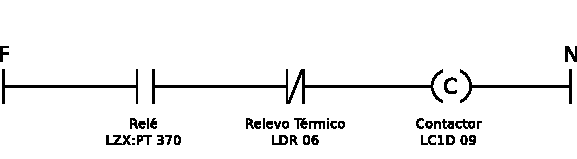
\includegraphics[scale=1.1]{Cap3-TableroElectrico/Images/ladderConexion.pdf}
 \caption{Esquema Ladder del conexionado de los motores.}
 \label{fig:diagramaLadderContactor}
\end{figure}

\subsection{Fuente de alimentación}
\label{subsec:fuenteAlim}
Los circuitos lógicos de la planta (\gls{plc}, sensores) funcionan con una
tensión de $24\,V$ de corriente continua.
Se optó por utilizar una fuente de alimentación industrial para energizar estos
circuitos lógicos.
Las características técnicas de la fuente son las siguientes:
\begin{center}
\begin{tabular}{|l|l|}
\hline
Marca & ReignPower\\
Tensión Entrada& $100-120$ / $200-240\,V$\\
Tensión Salida& $24\,V$\\
Corriente Salida Máxima& $4.2\,A$\\
Potencia & $100\,W$\\
\hline
\end{tabular}
\end{center}

En el diagrama de tablero, semuestran los conductores de $+24\,V$ y $0\,V$ en
rojo y negro respectivamente\todo{mantiene color?}.
La fuente de alimentación se muestra en el folio 1.

\section{Señal}
\label{sec:Senal}

El circuito de señal tiene como objetivos:
\begin{itemize}
 \item Relevar variables de la planta (caudal, presión), procesarlas y entregar
señales de control a la válvula electroneumática.
\item Activar los relés descriptos en la sección
\ref{subsec:alimentacionMotores} para encender o apagar los motores de las
bombas.
\item Conectar la planta a una computadora de control (\gls{scada}\todo{Esta
bien? Scada debería aparecer antes}), para poder
monitorear su estado como así también recibir señales de control.
\end{itemize}

\subsection{PLC}
\label{subsec:plc}

\glsreset{plc}
Para automatizar nuestra planta se optó por utilizar un \gls{plc}.
Se trata de un sistema electrónico digital de automatización y control, pensado
para aplicaciones industriales, seguro frente a condiciones adversas,
vibraciones\todo{buscar autómatas programables y sistemas de automatización
Mandado}, ruido electromagnético, etc \cite{bib:ApuntesJGabriel}.
El autómata se adapta al proceso a controlar mediante un
\textit{software} o programa de aplicación específico, que contiene la secuencia
de operaciones a realizar.
Pueden utilizar las entradas, los valores en memoria y valores
recibidos mediante un bus de comunicaciones del autómata para modificar el
estado de las salidas \cite{bib:libroAutomat1}.

Un \gls{plc} está conformado por los siguientes elementos:
\begin{itemize}
 \item \textbf{Procesador:} en función de las señales de los sensores
(entradas) y de la información almacenada, genera señales hacia los actuadores
(salidas).
El procesador sigue un algoritmo, denominado programa de aplicación,
que indica la secuencia de operaciones a realizar.
Entre los lenguajes de programación definidos en la norma \verb|IEC 61131|
podemos citar: Ladder, Texto Estructurado, Lista de Instrucciones y GRAFCET
(SFC).
 \item \textbf{I/O discretas:} las entradas y salidas discretas se
utilizan para acciones de control discretas, tal como encender motores
o leer sensores discretos (fin de carrera, por ejemplo).
En nuestro proyecto, se utilizan las salidas discretas \verb|Q0.0| y \verb|Q0.1|
para activar los relés de los motores.
Además \verb|I0.0| e \verb|I0.1| se
utilizan como señales de enclavamiento: conectadas a los contactores, verifican
que el motor se encuentre efectivamente encendido.
Se pueden observar estas señales de control en los folios 1 y 2 del diagrama de
tablero.
Además, se muestra el esquema de conexionado del \gls{plc} en el folio
3 del diagrama de tablero.
\item \textbf{I/O analógicas:} \todo{por qué es IW0.1.0?} Mediante una entrada
analógica, se pueden leer
señales de corriente ($4-20\,mA$) o tensión ($0-10\,V$) provenientes de los
sensores.
De la misma manera, las salidas analógicas permiten enviar consignas
de tensión o corriente a los actuadores.
En nuestro proyecto, las entradas analógicas \verb|IW0.1.0| e \verb|IW0.1.1|
permiten leer los valores de los DP cell de caudal y nivel, respectivamente.
Se emplea la salida analógica \verb|IW1.0| para controlar el
electroposicionador\todo[noprepend]{Verificad iw1.0}.
Cabe destacar que nuestro \gls{plc} no posee I/O analógicas.
Por ello, debió anexarse un módulo \verb|TWD AMM 6HT|.
Se pueden ver estas señales de control en el folio 4 del diagrama de tablero.
\todo[noline]{verificar orden, también en gráfico}

\item \textbf{Comunicación:} El puerto de comunicaciones permite programar el 
controlador, como así también enviar comandos y recibir información de
la planta durante la ejecución con el \gls{scada}.
El \gls{plc} utilizado cuenta con un puerto de comunicaciones \verb|RS 485|.
Se presentan dos opciones para la conexión con la computadora de control:
\begin{itemize}
 \item Mediante una conexión cableada:
 Conectamos el puerto \verb|RS 485| a un puerto \verb|RS 232| de la computadora
mediante un adaptador específico, fabricado durante el desarrollo del
proyecto\footnote{En nuestro caso, dado que la computadora no contaba con un
puerto serie, se utilizó un adaptador
\texttt{USB} a \texttt{RS 232}.}.
Se muestra en el anexo \ref{anexo:diag}, folio 6, el circuito esquemático
utilizado.
Además, en el anexo \todo{anexo}, se incluyen los diseños de PCB
para replicar el circuito.

No obstante, utilizar una conexión cableada impone un vínculo físico entre
el \gls{plc} y la computadora de control (impidiendo que la planta sea móvil).
\item Mediante un módulo de comunicación inalámbrica:
descripto en la sección \ref{subsec:inalambrico}.
\end{itemize}

\end{itemize}

\subsection{Módulos inalámbricos}
\label{subsec:inalambrico}

Para comunicar la planta con la computadora de control, sin necesidad de
utilizar un cable de par trenzado, se decidió utilizar un módulo inalámbrico
\verb|ADC-200| de CTM Electrónica.
Se trata de un equipo de comunicaciones para realizar enlaces inalámbricos que
utilicen la interfaz \verb|RS 232| o \verb|RS 485|.
Podemos citar, entre las características técnicas relevantes:

\begin{center}
\begin{tabular}{|l|l|}
\hline
Alimentación & $5\,VCC$\\
Consumo& $60\,mA$\\
Alcance& $1000\,m$\\
Baud Rate &2400 a 19200 bps \\
Frecuencia& 431 a 470 Mhz en más de 100 canales\\
\hline
\end{tabular}
\end{center}

Para el proyecto, se conectó el módulo tal como lo indica el
diagrama de tablero (folio 5), estipulando una velocidad de transferencia de
\verb|xxxx bps|, sin pariedad\todo{verificar velocidad y paridad}.

Además, dado que el módulo inalámbrico debe alimentarse con una tensión de
$5\,V$ de corriente continua, se desarrolló una fuente conversora de $24\,V$ a
$5\,V$ basada en el integrado \verb|LM7805|.
El circuito esquemático de la fuente puede encontrarse en el folio 7 del anexo
\ref{anexo:diag}.
Además, se incluye el diseño del PCB en el anexo \todo{anexo} para poder
replicar el circuito.

Cabe destacar que el módulo inalámbrico \textbf{no puede utilizarse} para
la programación del \gls{plc}, debido a que el software (Twido) acusa un error
de timeout.
No obstante, su funcionamiento es correcto para recibir información
del estado de la planta y enviar consignas mediante el \gls{scada}.

\section{Imagen del tablero}
En la imagen \ref{fig:fotoTablero} \todo{incluir una foto del tablero}se muestra
una fotografía del tablero finalizado. 
Pueden observarse tres niveles diferenciados:
\begin{itemize}
 \item En el nivel superior se encuentra el interruptor termomagnético de corte
general descripto en la sección \ref{subsec:alimentacionMotores}.
Este interruptor debe ser accionado para encender la planta.
\item En el nivel medio se encuentran los relés, contactores y relevos térmicos
para accionar los motores de las bombas (sección
\ref{subsec:alimentacionMotores}).
\item En el nivel inferior está la fuente de alimentación de $24\,V$ (sección
\ref{subsec:fuenteAlim}) y el
\gls{plc}, con su módulo de E/S analógicas (sección \ref{subsec:plc}).
\end{itemize}
Los elementos fueron montados sobre
rieles DIN.  Además, todos los elementos (a excepción del interruptor
termomagnético) se encuentran protegidos por un acrílico transparente para
evitar accidentes.

\begin{figure}[ht]
 \centering
 \missingfigure{foto tablero}
 \caption{Fotografía del tablero finalizado}
 \label{fig:fotoTablero}
\end{figure}
